\documentclass{article} %选择文档类型,我们如果是做期末大作业的话选article就可以了
\usepackage{anyfontsize}
%正如c++需要import库来实现各种各样的功能,Latex也需要调用宏包来实现各种各样的功能
\usepackage{amsmath}  %调用公式宏包
\usepackage{graphicx} %调用插图宏包
\graphicspath{{code_Latex/}}
\usepackage{ctex}     %调用中文宏包
\usepackage{float}
\usepackage{cite}


%\begin{document}这句话之前是导言区,这句话以后就开始写正文了
%可以把导言区理解为int main()函数之前的内容,而正文就是int main()主函数的部分了
\usepackage{geometry}
\geometry{left=1.5cm,right=0.5cm,top=1.0cm,bottom=1.5cm}

\begin{document}
    \title{\centerline{数逻实验四报告}}
    \date{大二秋 实验四:状态机}
    \author{信息学部计算机与电子通信7班 2023311704 王昕远 t2 612}
    \maketitle
    \thispagestyle{empty}


\section{状态机}

信号说明:时钟信号clk,数据有效信号valid,复位信号rst,需要发送的数据data[7:0],输出信号dout\par
定义四个状态:IDLE,START,DATA,STOP\par
波特率信号:baud\_tick\par
\section{仿真图像分析}
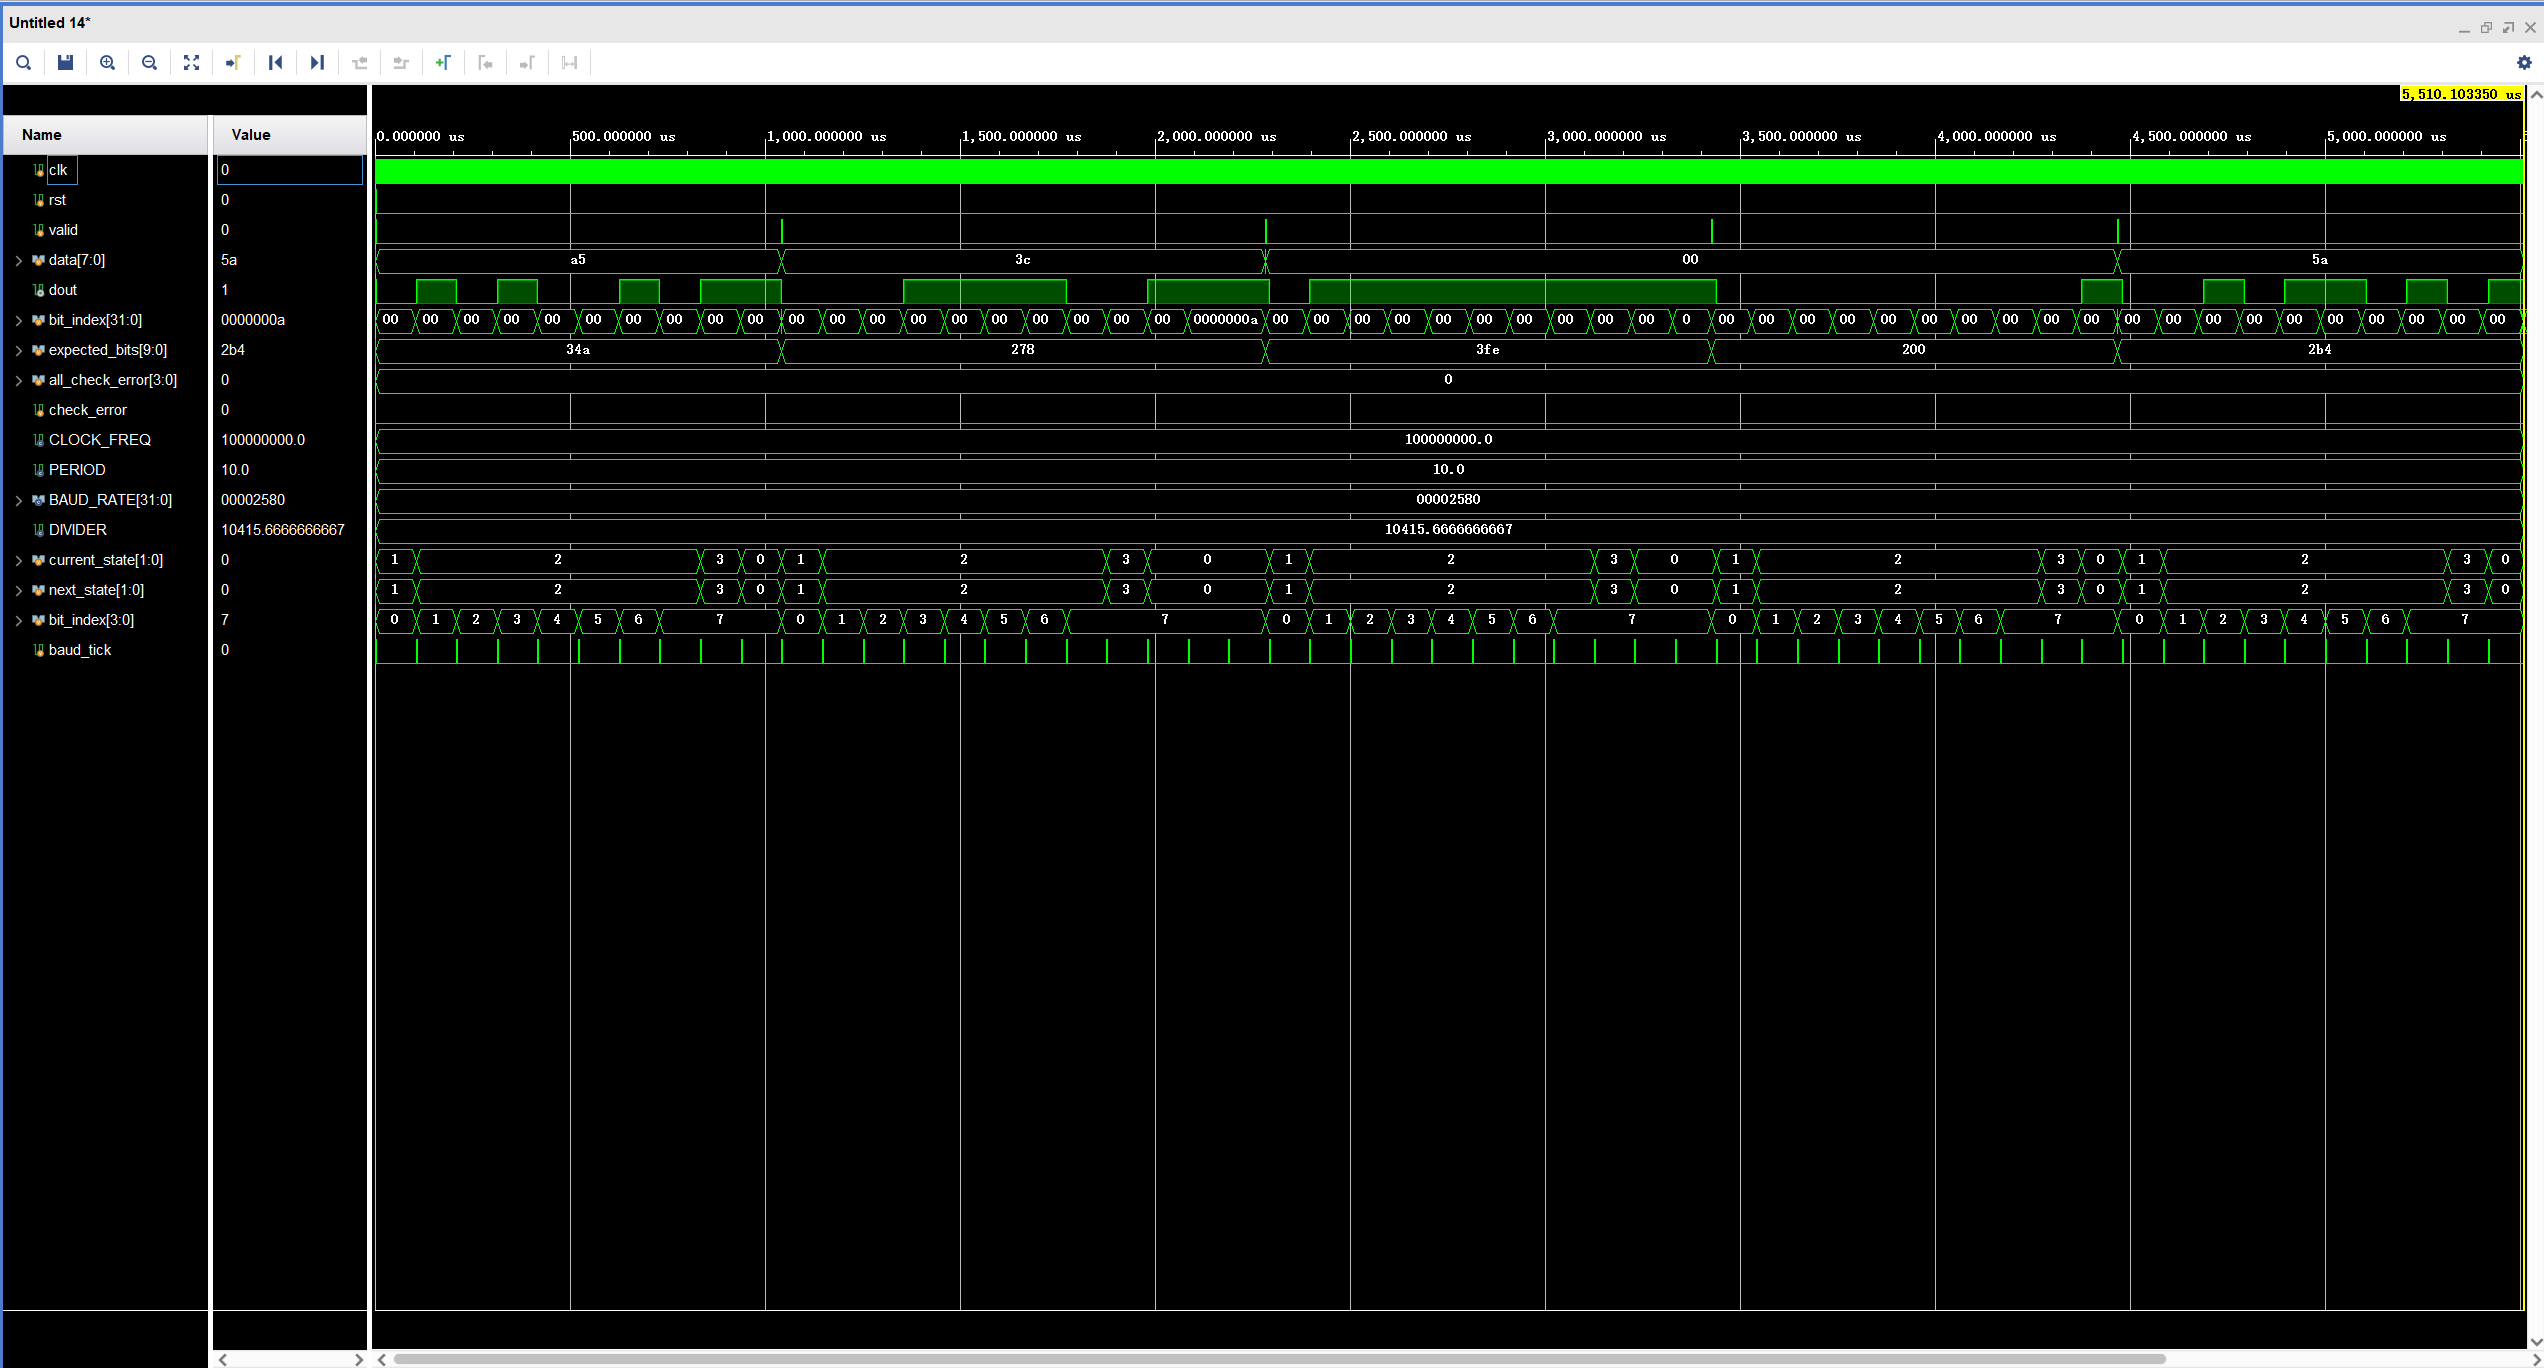
\includegraphics[width=0.8\textwidth]{1.png}\par
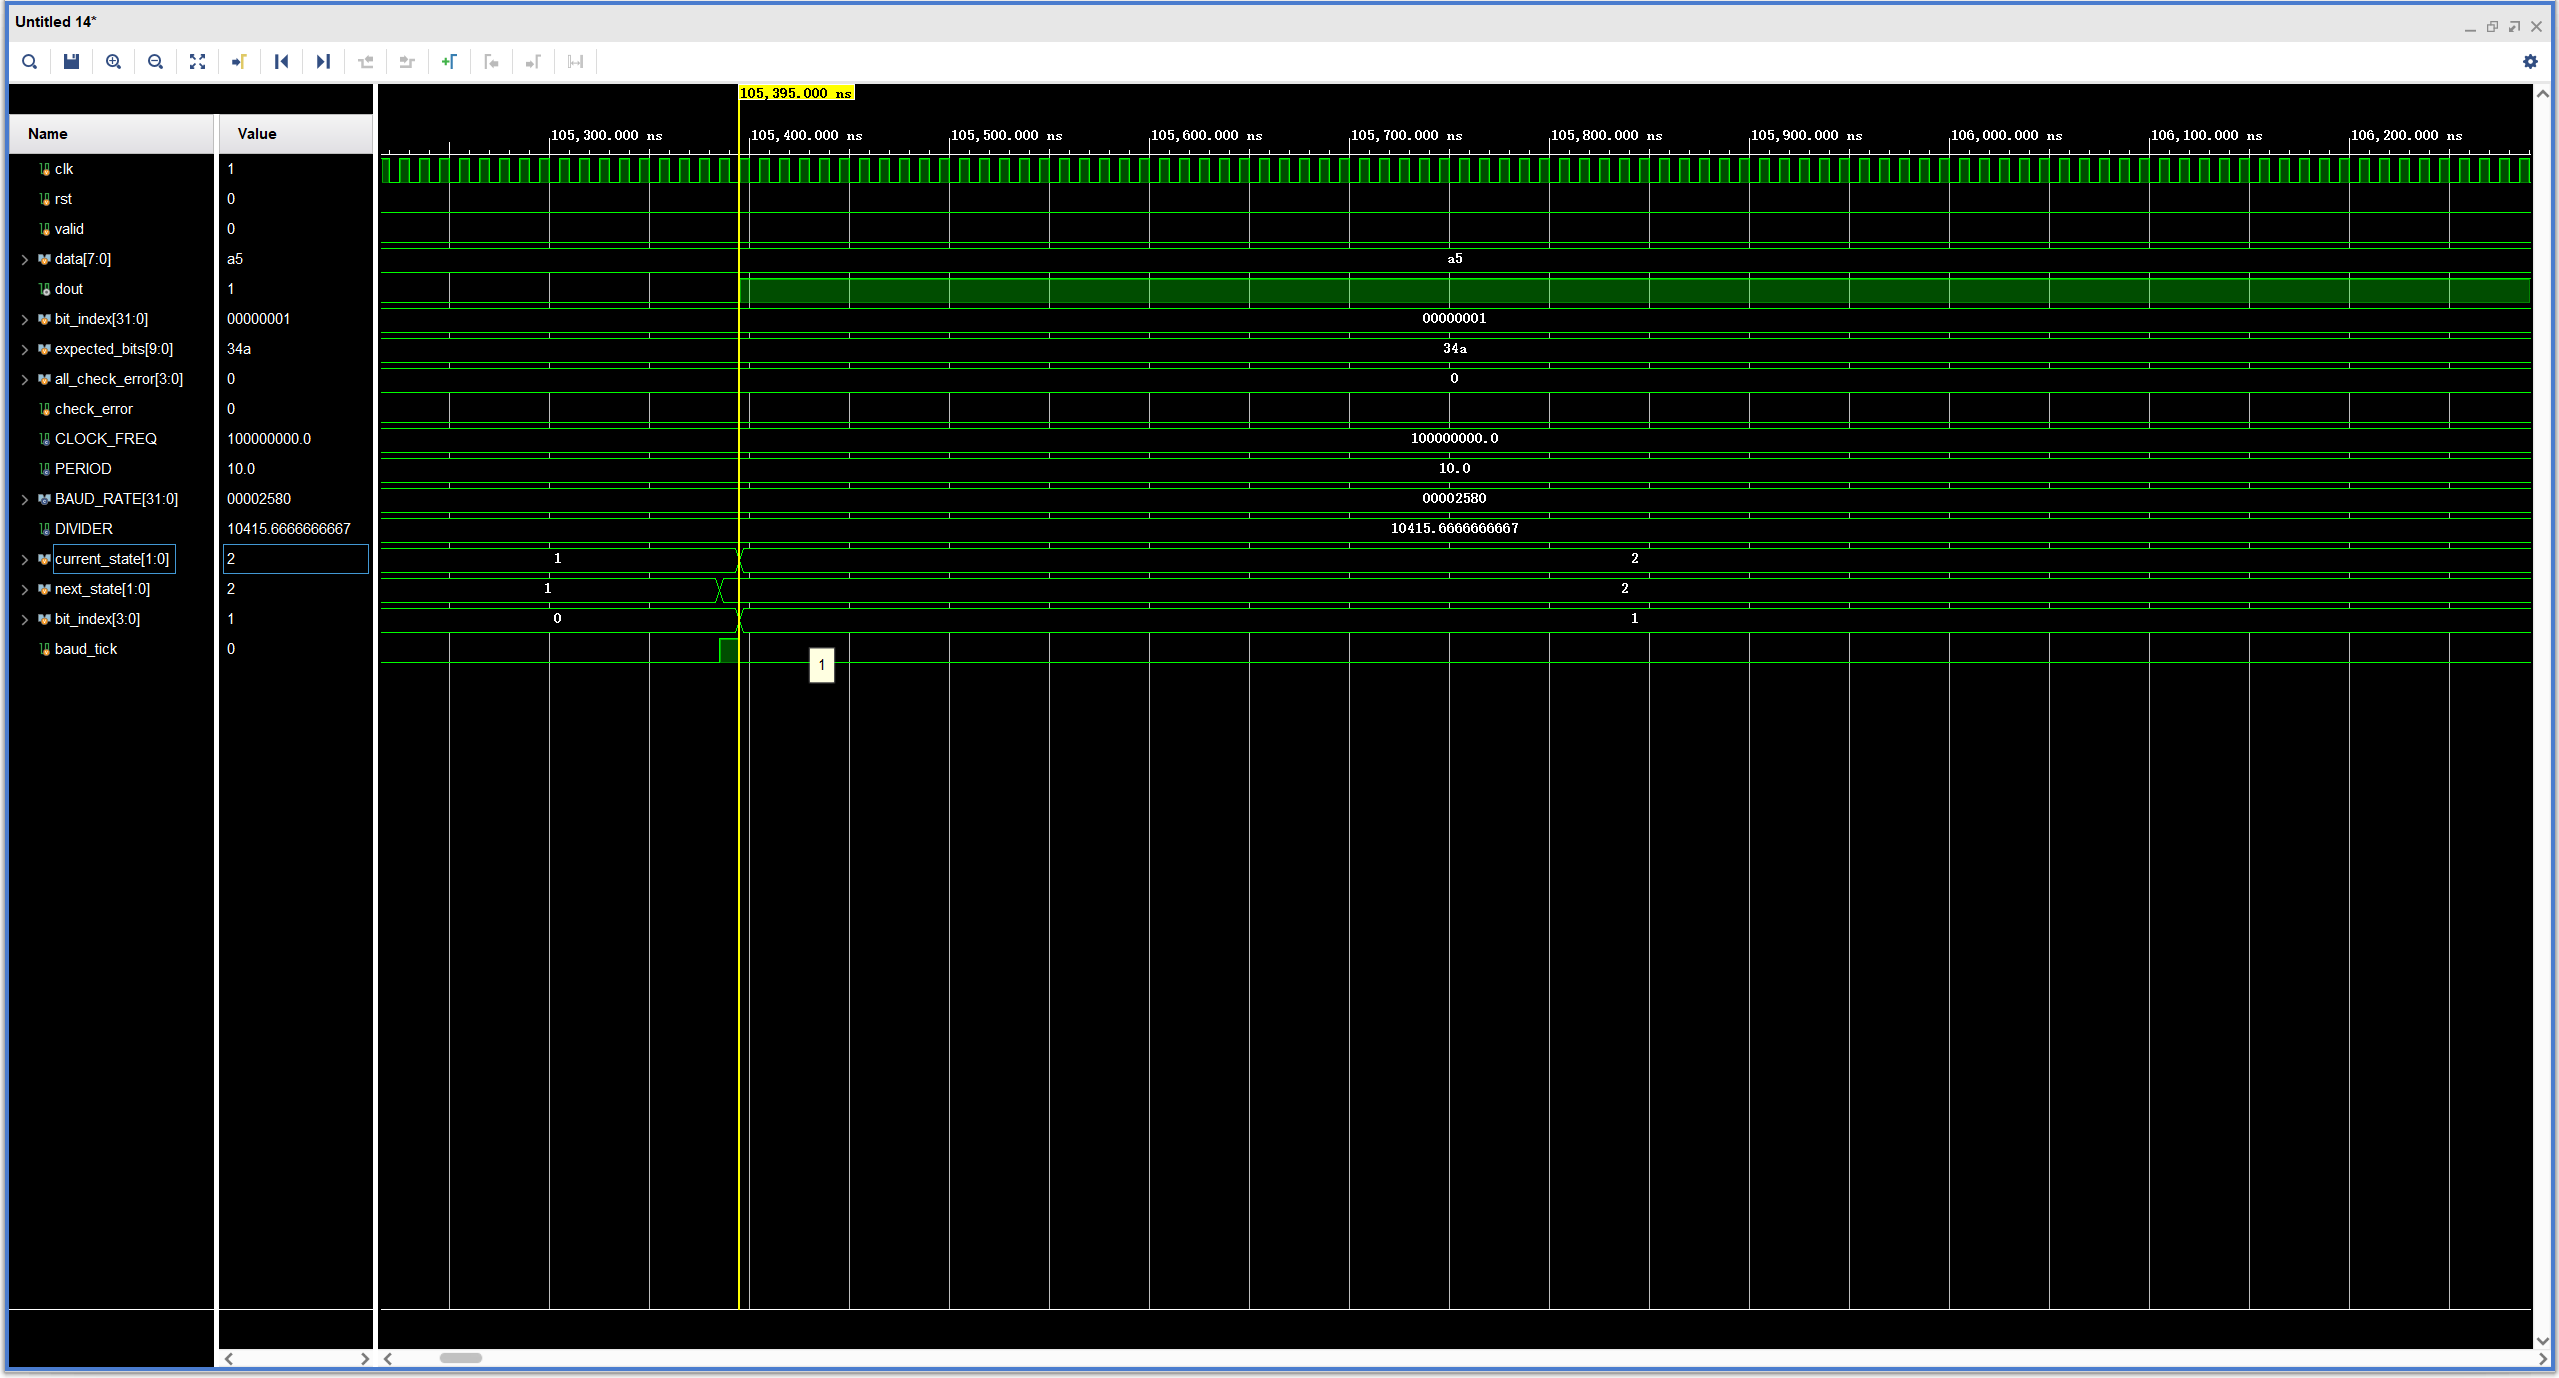
\includegraphics[width=0.8\textwidth]{2.png}\par
总共测试了五个样例,有五个valid有效输入,约定波特率为9600.\par
输入为data变量,逐位输出为dout信号,每个baud周期输出一位\par
current\_state为现态,next\_state为次态,两者变化相差一个clk周期\par
四个状态对应不同输出。IDLE状态为默认状态,输出高电平1,START为开始状态,第一位输出,输出信号为低电平0,DATA为输出数据,从低到高输出依次8位数据,STOP为停止,输出高电平1。\par
状态依次进行转换,变化周期为1个约定的周期。\par

\section{状态转移图}
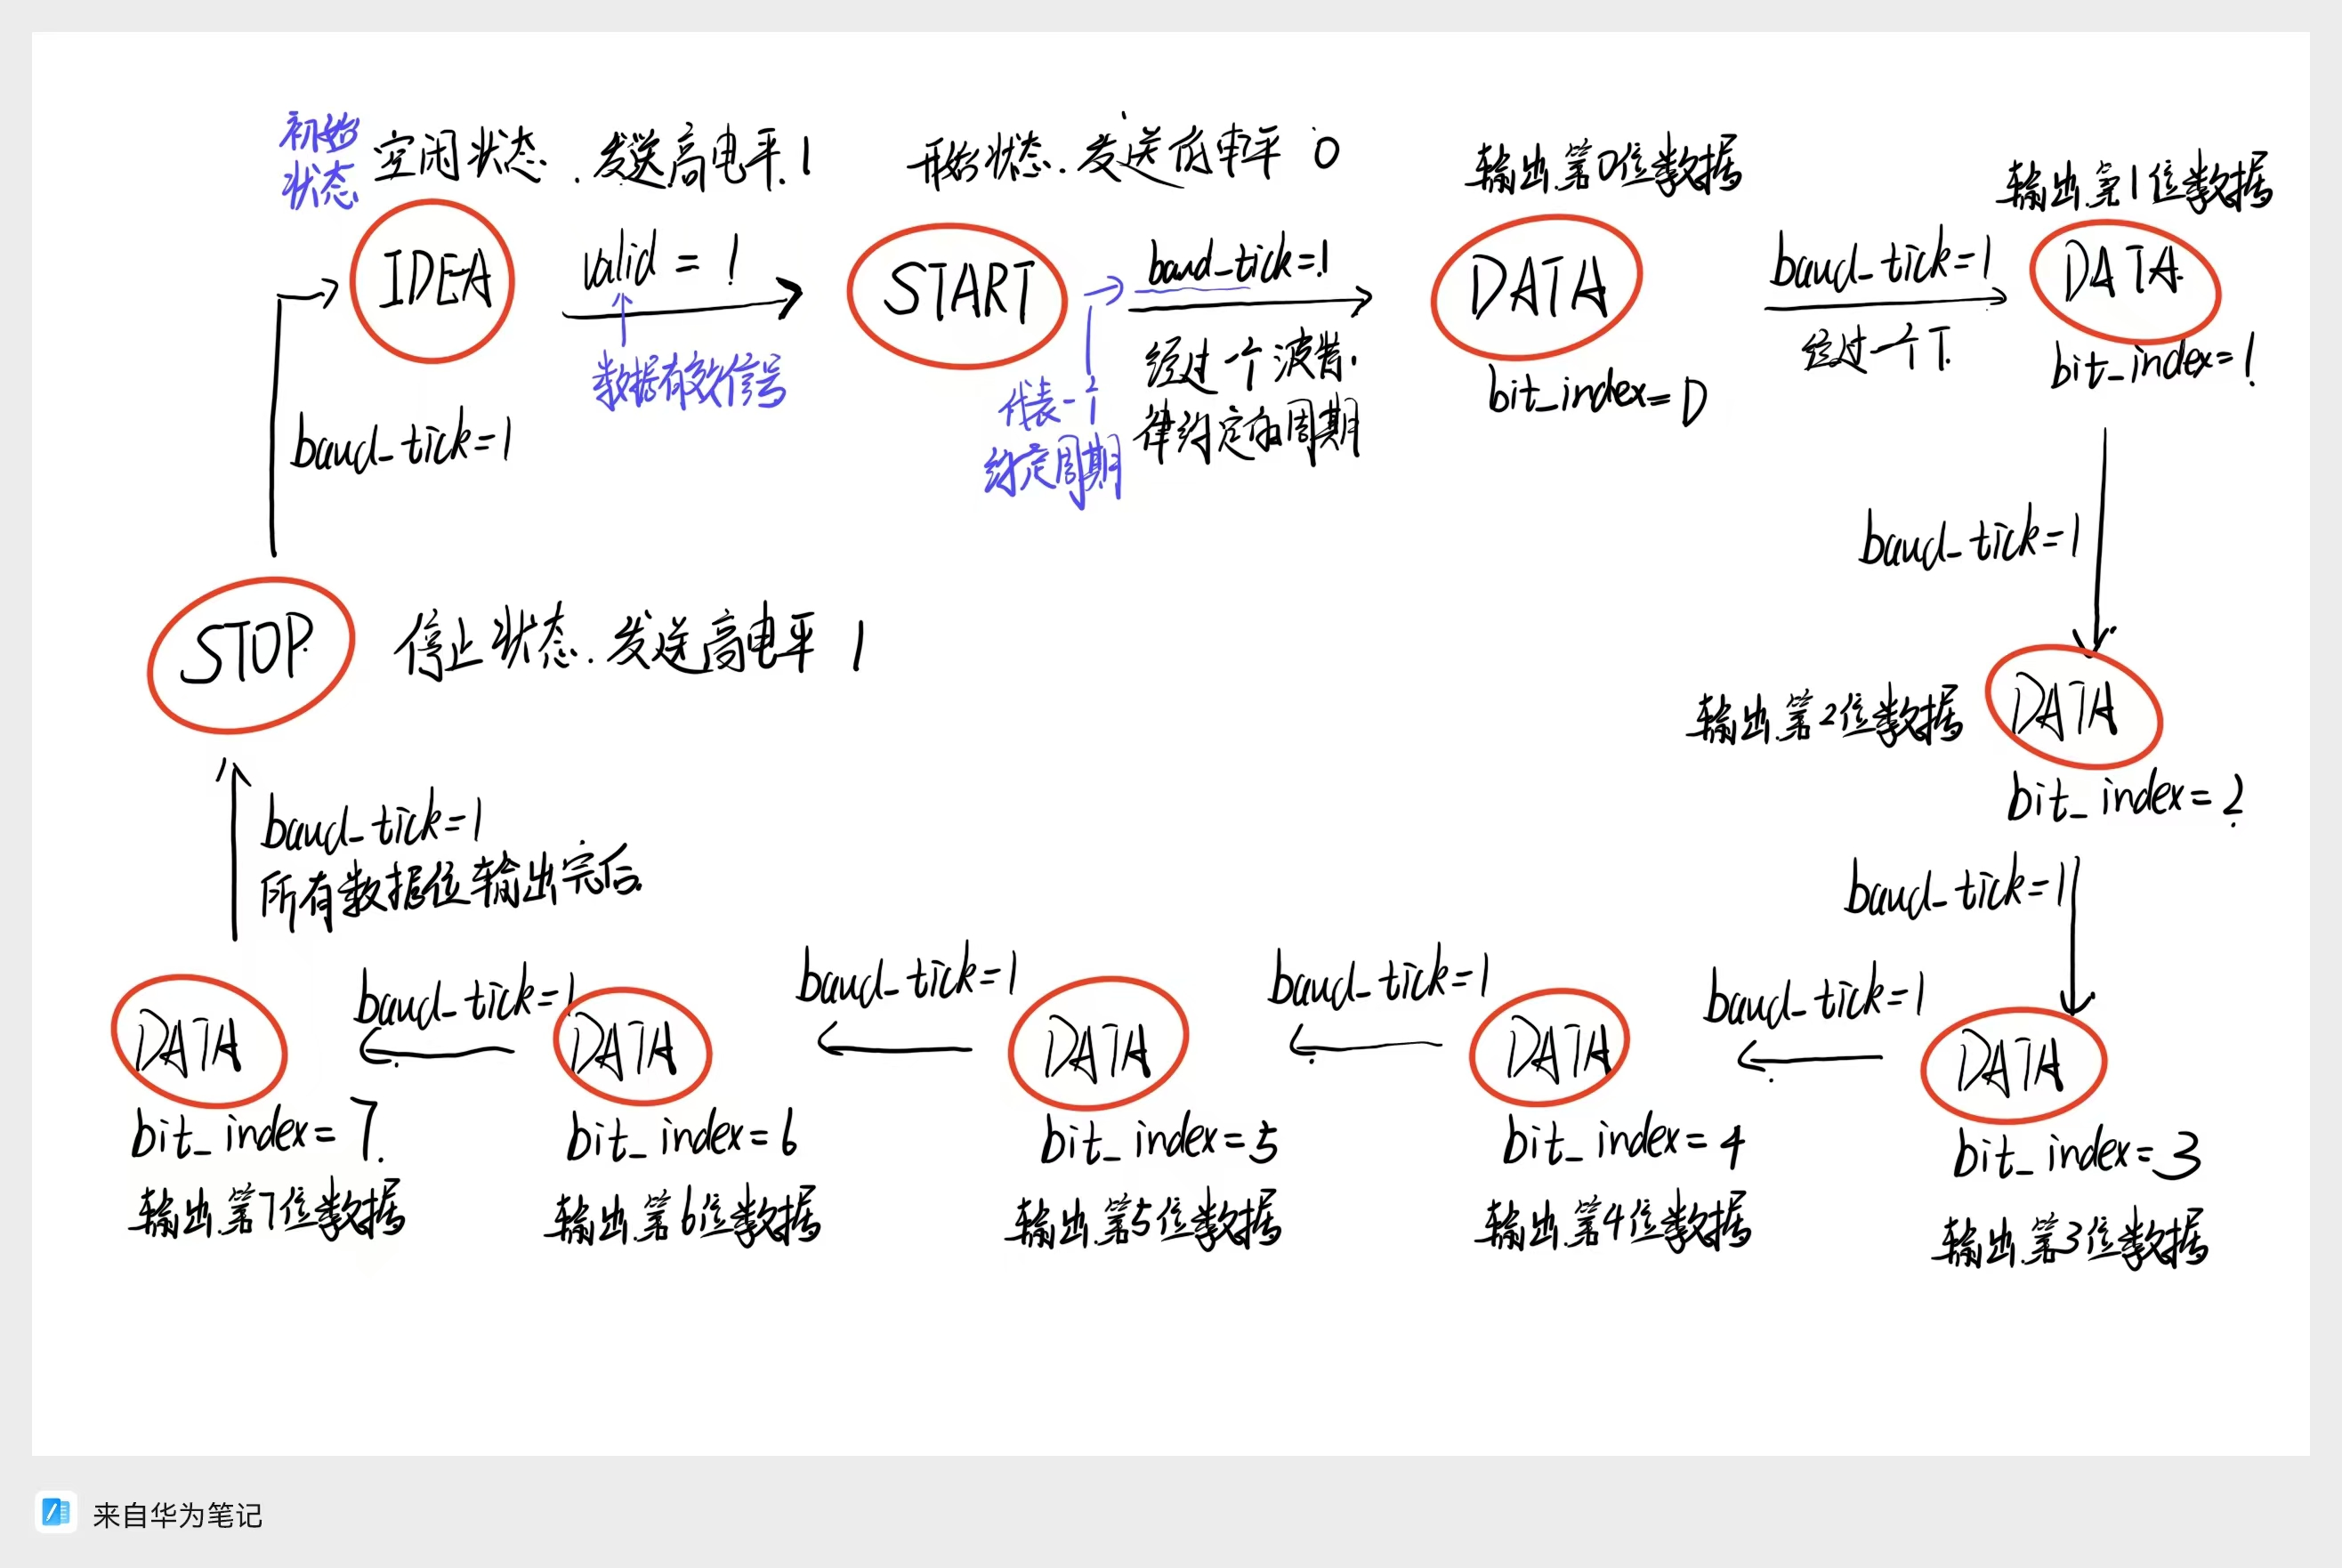
\includegraphics[width=0.8\textwidth]{22.jpg}\par

\section{RTL图分析}
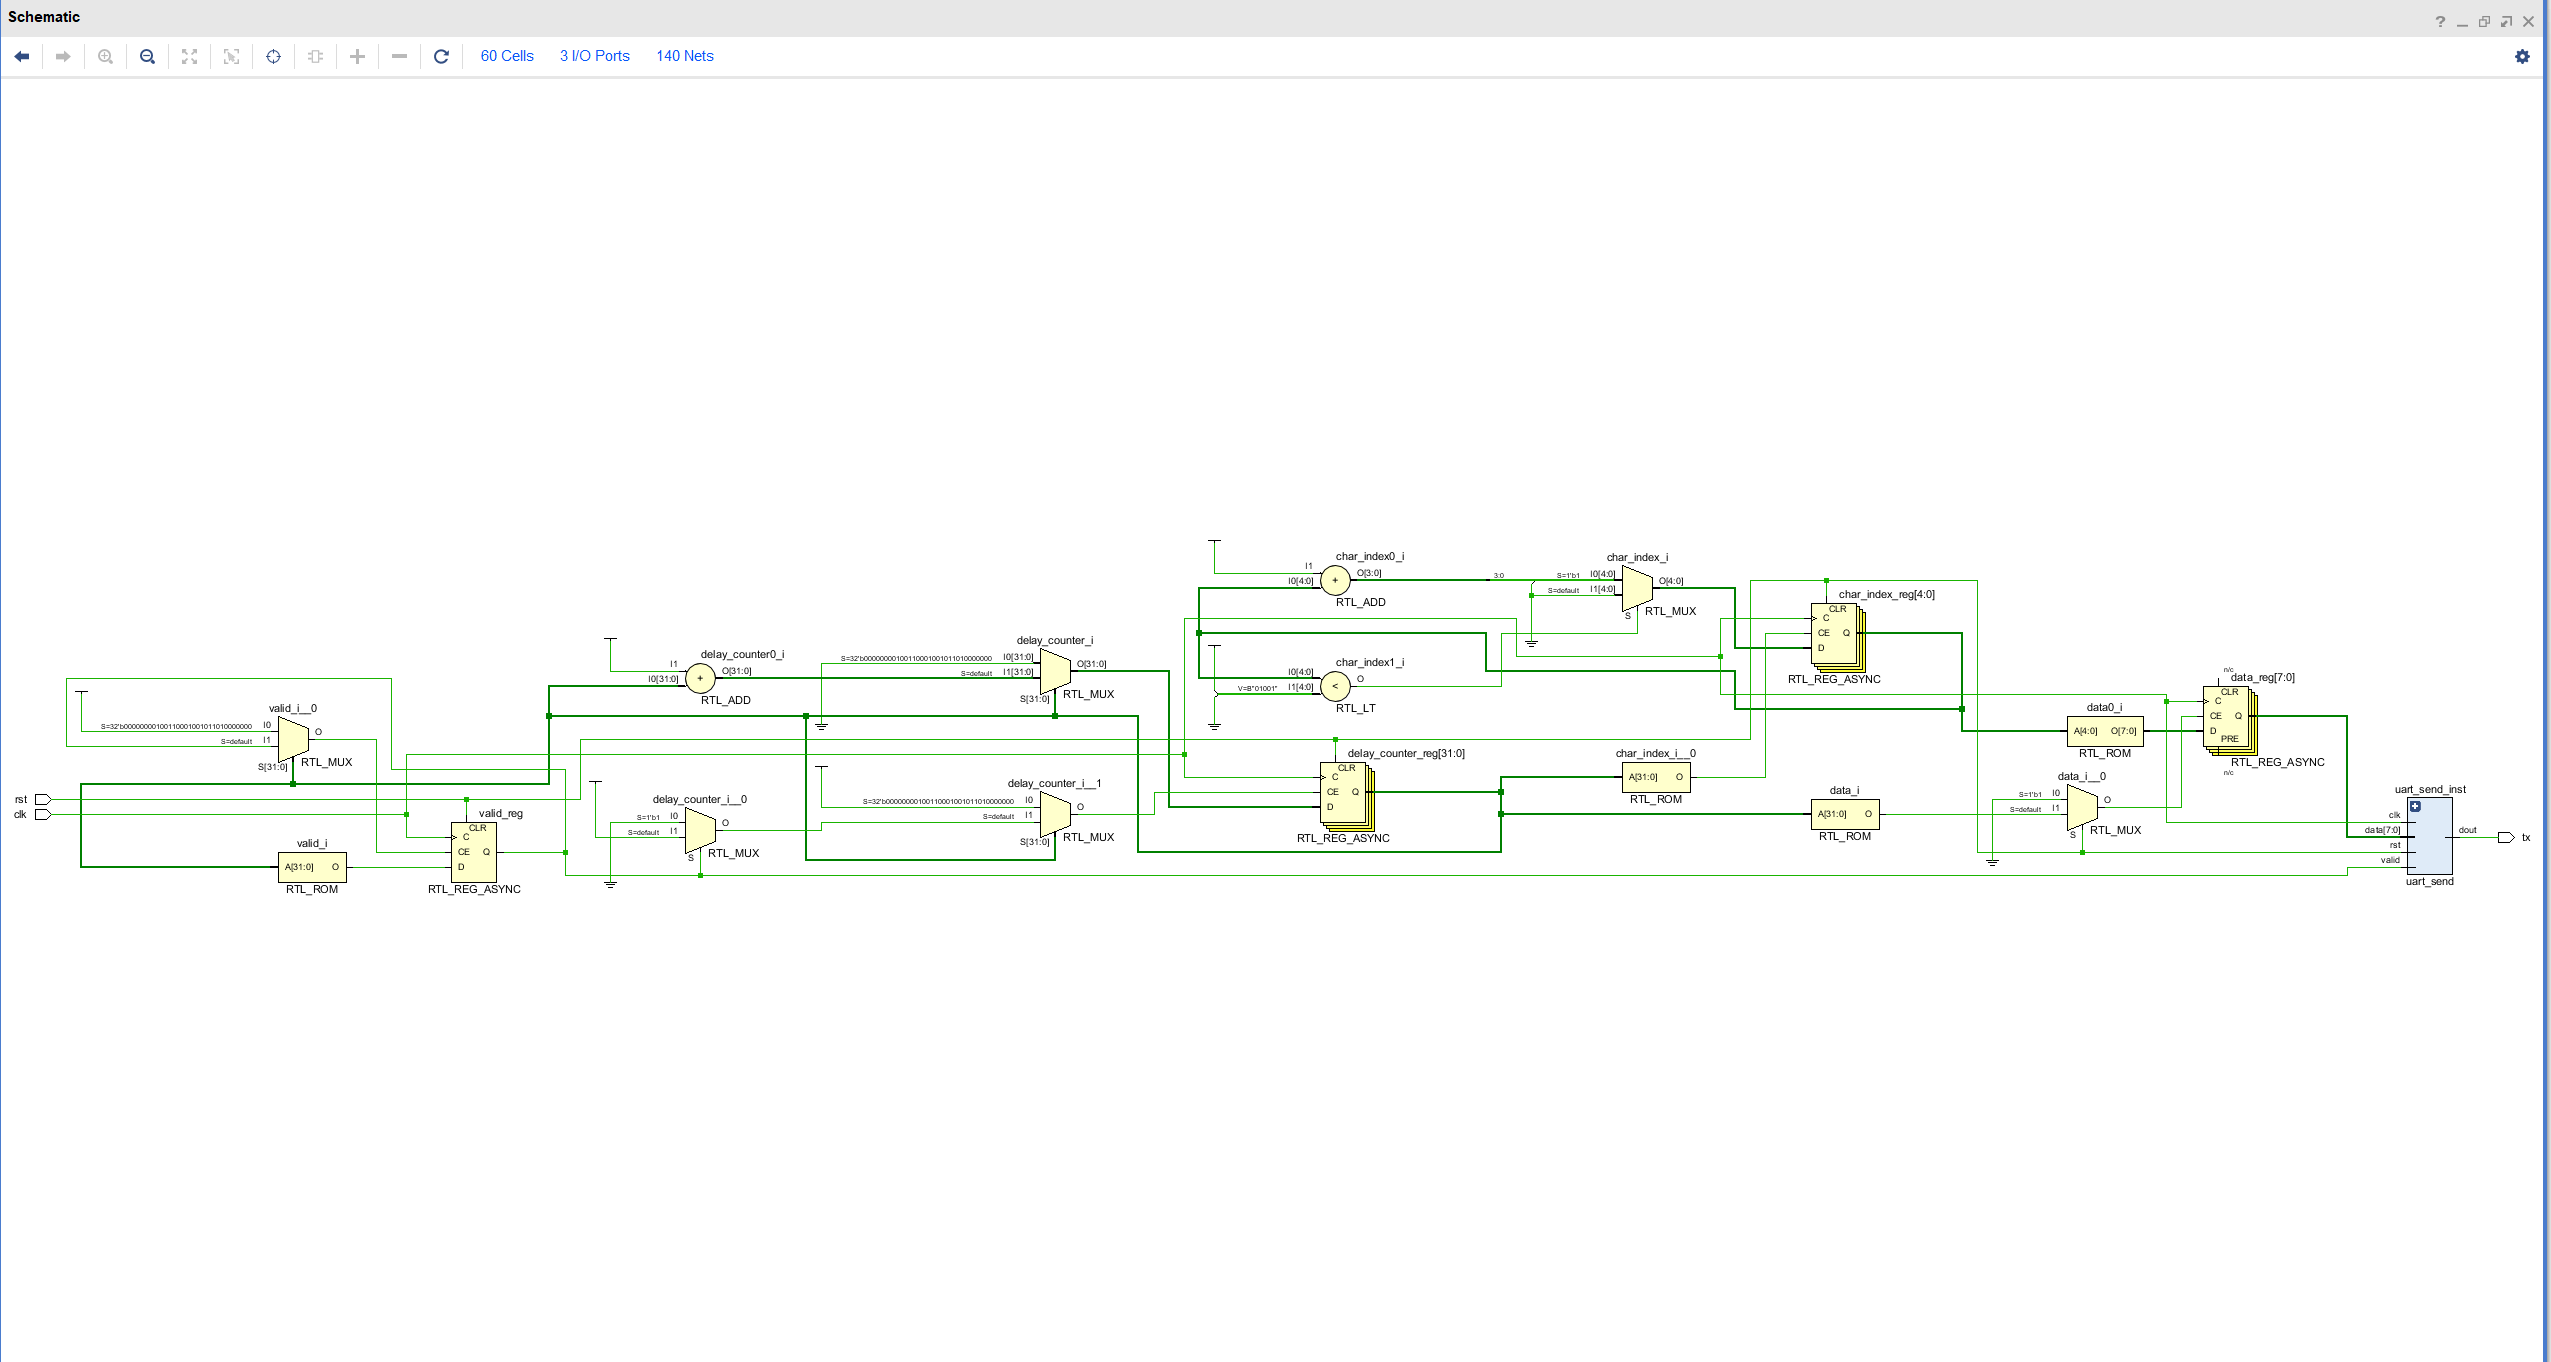
\includegraphics[width=0.8\textwidth]{RTL.png}\par
该图为RTL电路图,构成状态机电路。\par
$$
$$
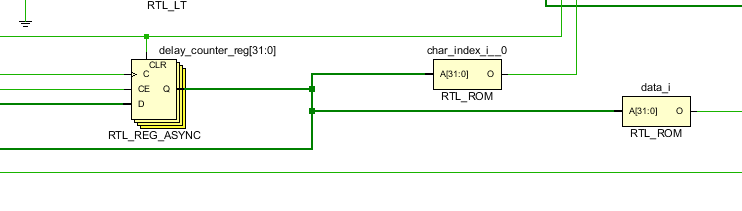
\includegraphics[width=0.45\textwidth]{11.png}
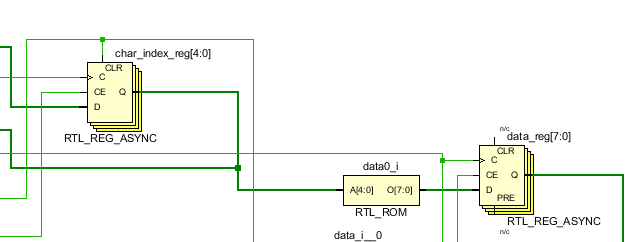
\includegraphics[width=0.45\textwidth]{111.png}\par
该位置是状态寄存器\par
$$
$$
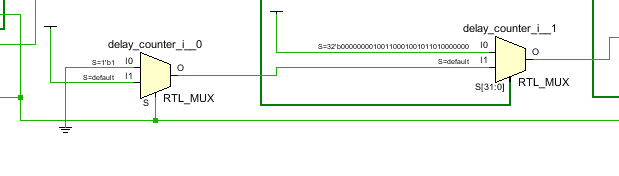
\includegraphics[width=0.5\textwidth]{12.png}\par
该位置是转移逻辑电路\par
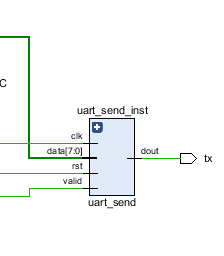
\includegraphics[width=0.5\textwidth]{13.png}\par
该位置是输出电路\par

\end{document}